\documentclass[aps,rmp,reprint,superscriptaddress,notitlepage,10pt,onecolumn]{revtex4-1}
\usepackage[utf8x]{inputenc}
\usepackage{amsmath,amsthm,amsfonts,amssymb,amscd}
\usepackage{graphicx}
\usepackage{wrapfig}
\usepackage{enumerate}
\usepackage[final]{hyperref}

\newcommand{\avg}[1]{\langle #1 \rangle}

\graphicspath{{../figs_suppl/}{./figs_suppl}}

\begin{document}
\title{PanGraph: scalable bacterial pan-genome graph construction \\ Supplementary Information}
\author{Nicholas Noll}
\affiliation{Kavli Institute for Theoretical Physics, University of California, Santa Barbara \looseness=-5}
\author{Marco Molari}
\affiliation{Swiss Institute of Bioinformatics, Basel, Switzerland \looseness=-5}
\affiliation{Biozentrum, University of Basel, Basel, Switzerland \looseness=-5}
\author{Richard A.~Neher}
\affiliation{Swiss Institute of Bioinformatics, Basel, Switzerland \looseness=-5}
\affiliation{Biozentrum, University of Basel, Basel, Switzerland \looseness=-5}

\maketitle

\section{Generation of synthetic data}

As a first test we benchmark the performances and accuracy of \textit{PanGraph} on synthetic data, obtained by simulating the evolution of a population in which individuals can loose part of the sequence from deletions, or gain new genetic material via Horizontal Gene Transfer (HGT) from other members of the population.\\
In the simulation a population of size $N$ is evolved for $T$ generations using a Wright-Fisher model \cite{hudson2002generating}. Each individual in the population has a circular genome of initial size $L$. At each generation mutations occur at a rate $\mu$ per position per generation.\\
Deletions can occur at a rate $d$ per genome per generation. When a deletion is suggested on isolate $n$, having a genome length $L_n$, a new desired length $L'_n$ is extracted from a Gaussian distribution with mean $L$ and variance $\sigma^2$. If $\Delta = L'_n - L_n < 0$ then a random chunk of length $|\Delta|$ is removed from the genome, reducing it to size $L'_n$. If $\Delta > 0$ no deletion is performed. This ensures that the length distribution of genomes in the population remains close to the desired length $L$, with $\sigma^2$ being a proxy for the variance.
HGT occurs at a rate $h$ per genome per generation. Similarly to deletions, when a HGT event is suggested a new desired length $L'_n$ is extracted from the same Gaussian distribution, and this time the event is performed only if $\Delta = L'_n - L_n > 0$. In this case a random chunk of sequence of length $\Delta$ is extracted from a random individual in the parent population (possibly the parent of isolate $n$ itself) and inserted in a random position of the genome of isolate $n$.
Finally, inversions occur at a rate $i$ per genome per generation. When an inversion is proposed a random length $\Delta$ is chosen in the same way, and a random chunk of length $|\Delta|$ is inverted.
Standard values of the simulation parameters are reported in Table~\ref{table:sim-params}.

\begin{table}[hb]
    \begin{tabular}{c l l}
    \hline\hline
    Parameter & Description & Standard Value \\
    \hline
    $N$ & population size & 100 \\
    $T$ & n. of simulated generations & 50 \\
    $L$ & average genome size & $5 \cdot 10^5$ [bp] \\
    $\sigma$ & s.t.d. of genome size & $L/10$ [bp]  \\
    $\mu$ & mutation rate & 0.005 [1/bp $\cdot$ generation] \\
    $d$ & deletion rate & 0.05 [1/generation] \\
    $i$ & inversion rate & 0.01 [1/generation] \\
    $h$ & HGT rate & 0.1 [1/generation] \\
    \hline
    \end{tabular}
    \caption{{\bf Simulation parameters}. Description of all simulation parameters used for the generation of synthetic data. Unless otherwise specified, the standard value is used.}
    \label{table:sim-params}
\end{table}

At the end of the simulation the resulting mosaic genomes are collected, along with the real underlying pangenome graph that can be used as the ground truth against which to check the performances of \textit{PanGraph}. The code to perform these simulations is shipped with \textit{PanGraph} in the \verb|generate| command.

\section{Benchmark of \textit{PanGraph} on synthetic data}

We test the performance of \textit{PanGraph} on synthetic data generated with the simulation described above. We focus on two aspects: the computational performances of the algorithm (time and memory requirements) as a function of the dataset size, and the accuracy of the algorithm in reconstructing the real pangenome graph of the population as a function of sequence divergence.

\subsection{Computational performance}

To test the computational performances of \textit{PanGraph} we generated data using the model described in the previous section, with standard value of the parameters but varying the average genome length $L=[1,5,10,50,100,500]$ kbp and the population size $N=[10,20,50,100,200,500,100]$. For each pair of $N,L$ values we generated 50 different datasets. On each dataset we ran the \textit{PanGraph} \verb|build| command, using \textit{minimap2} as alignment kernel with \textit{asm20} option. We used standard value for the energy parameters $\alpha=100$, $\beta=10$. Runs were performed using 8 cores. For each run we measured the wall-time of the command, the maximum memory requirements (maximum resident size) and the average cpu percent. Results are displayed in Fig.~\ref{fig:benchmark-perf-suppl}.
Thanks to the guide tree architecture of \textit{PanGraph} the run time scales almost linearly with the number of isolates.

\begin{figure}[h]
    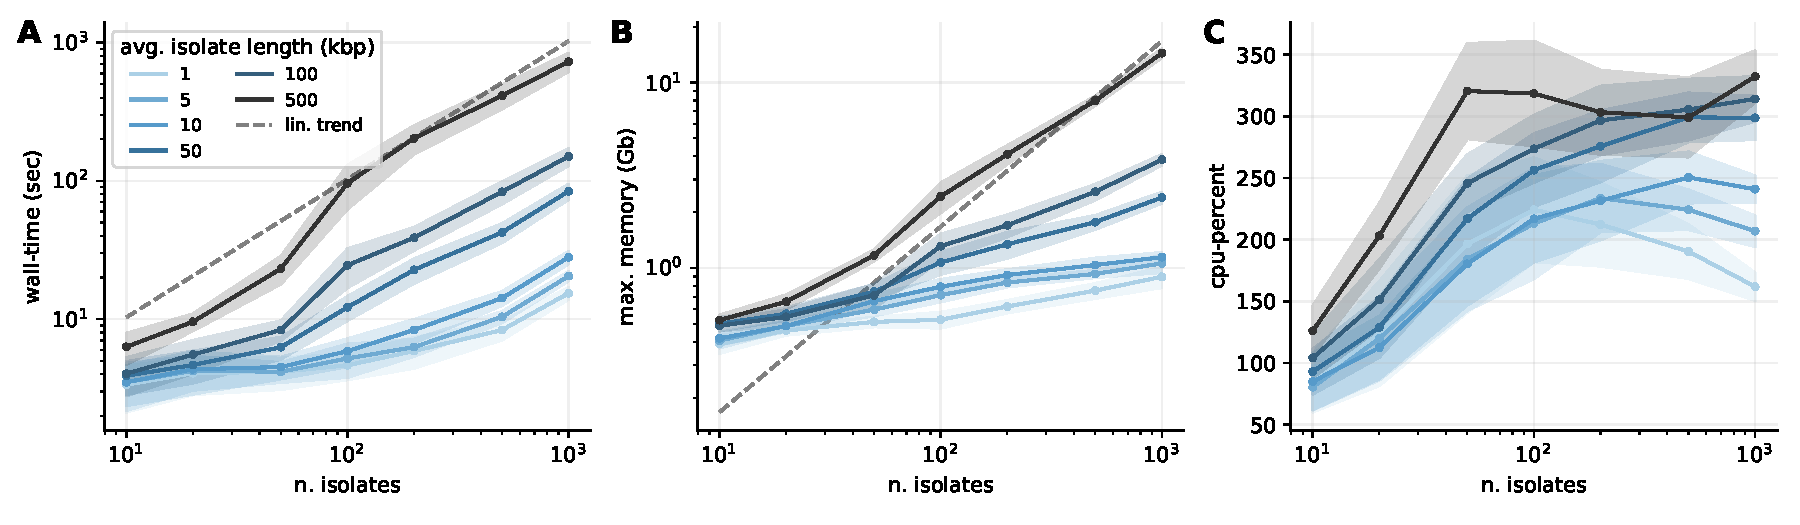
\includegraphics[width=.9\textwidth]{figs_suppl/benchmark_suppl.pdf}
    \caption{{\bf Computational performance of PanGraph algorightm on synthetic data, as a function of dataset size}. We run PanGraph on artificially generated datasets consisting of a variable number of isolates with genomes of variable length (colorscale). For each condition we display the average and standard deviation over 50 different runs of: (A) algorithm wall-time, (B) maximum memory requirement and (C) average percentage of cpu used on a total of 8 cores.}
    \label{fig:benchmark-perf-suppl}
\end{figure}


\subsection{Accuracy in reconstructing the pangenome graph}

To test the accuracy of \textit{PanGraph} in reconstructing the pangenome graph of a set of isolates we generated artificial data using the procedure described above, obtaining both a set of genome sequences and the underlying real pangenome graph. This was done using standard value of the parameters, but varying the rate of HGT in the interval $h=[0.01,1]$ and the mutation rate $\mu=[0,0.01]$. For each $(h,\mu)$ pair 25 different set of data were generated.\\
On each set of data we executed \textit{PanGraph} with values for the energy parameters $\alpha=0$ and $\beta=0$, and with three different alignment kernels:
\begin{itemize}
    \item \textit{minimap2} with option \textit{asm10}
    \item \textit{minimap2} with option \textit{asm20}
    \item \textit{mmseqs2}
\end{itemize}
Thus obtaining three different pangenome graphs per dataset.\\
To link the mutation rate parameter $\mu$ with the average pairwise SNPs distance $\avg{d}$ between homologous segments in the population we evaluated the average pairwise distance for every pancontig in the pangenome graph comprising more than a single path. For each graph we then perform the weighted average of the divergences, using as weight the length of the panconting. Finally, for every pair of parameters $(\mu,h)$ we average these numbers over the 25 different simulations. Results are displayed in Fig.~\ref{fig:snps-suppl}.\\
While the rate of HGT does not influence the average pairwise divergence of pancontigs, the choice of alignment kernel controls their maximum divergence. \textit{Minimap2} is able to correctly merge pangenome graphs with up to $\avg{d} \sim 7\%$ with the \textit{asm20} option, while \textit{mmseqs2} reaches $\avg{d} \sim 10\%$ at the expense of higher time requirements.\\
By performing a linear fit on the datapoints with $h \leq 0.002$ we are able to recover the conversion factor between the HGT rate and average pairwise divergence of pancontigs in our simulations: $\avg{d} \sim 20.8 \, h$.

\begin{figure}[h]
    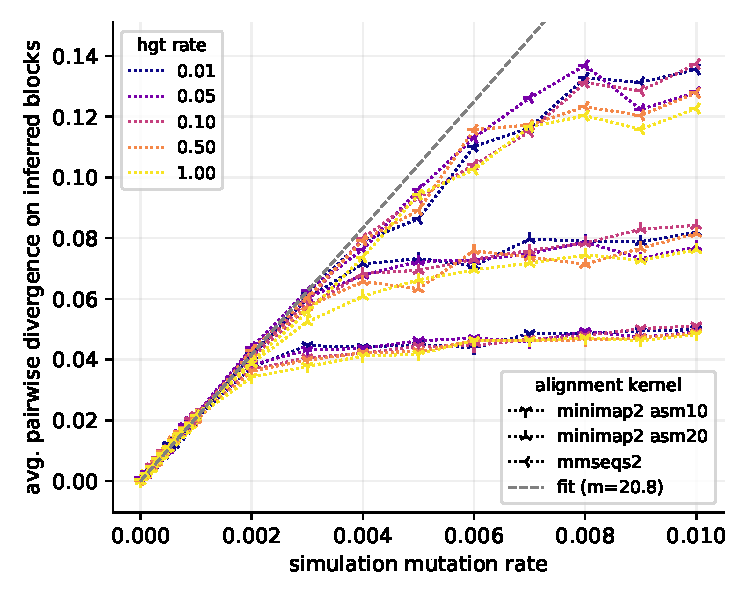
\includegraphics[width=0.5\textwidth]{figs_suppl/snps_rate_vs_divergence.pdf}
    \caption{{\bf mutation rate vs divergence on synthetic data}. We compare the mutation rate $\mu$ of our simulations with the average pairwise divergence of sequences in pancontigs of the resulting pangenome graphs. This is done for different values of the rate of HGT $h$ and for three different alignment kernels. As expected, the divergence is only marginally influenced by the HGT rate, but the saturating value of the divergence depends strongly on the choice of alignment kernel, with \textit{mmseqs2} being able to merge sequences with average divergence higher than 10\%. To find the relationship between the mutation rate $\mu$ and the average pairwise divergence of the sequences we peform a linear fit on data points for $\mu \leq 0.002$. This provides the conversion factor $\avg{d} \sim 20.8 \, \mu$.}
    \label{fig:snps-suppl}
\end{figure}

Once this link has been established we group simulations by the value of $h$ and check for accuracy comparing the reconstructed pangenome graphs with the ground truth provided by our simulation. In particular for each isolate we consider the breakpoints between different pancontigs that tile the genome, and measure the displacement between the real position of these breakpoints and the position reconstructed by pangraph.\\
To evaluate this displacement it is first necessary to link breakpoints on the real and reconstructed pangenome graph. We formulate this problem as an assignment problem, and solve it numerically using the Hungarian method \cite{kuhn1955hungarian}. For each isolate we call $b_i$ for $i=1,\ldots,I$ the panconting breakpoints on the real pangenome graph, and $b_j$ for $j=1,\ldots,J$ the ones on the reconstructed pangenome graph.\footnote{To avoid artifacts generated by the default threshold distance $d=100$ bp of pangraph, if on any of the two pangenome graphs a pair of breakpoints sits at a distance smaller than this threshold, we remove one of them from the set of breakpoints.} We define a cost matrix $D_{ij} = d(b_i,b_j)$ whose elements are distances on the genome of the isolate of pairs of breakpoints on the two graphs. We then numerically solve the assignment problem on this matrix, and obtain a set of $K = \min\{ I,J \}$ pairings between breakpoints such that the distance between the pairs is minimal and all the breakpoints of the graph with minimum number of breakpoints have been paired. The average distance between breakpoints in these pairs is the average breakpoint distance of the graph.\\
For each simulation we obtain a number of average breakpoint distances equal to the number of isolates in the simulation. In Fig.~\ref{fig:benchmark-accuracy-suppl} we plot the cumulative distribution of these distances, considering only distances smaller than 1 kbp, stratifying simulations according to the average pairwise divergence of pancontigs inferred from the value of $\mu$. Each panel correspond to a different alignment kernel. As the sequence diversity increases we observe a clear transition. For low diversity most of the breakpoints are inferred to be only a few bp away from their real position, while for highly diverged sequences the position of breakpoints is not precisely inferred and can be hundreds of bp away from their real position. For different alignment kernels this transition occurs at different values of the divergence, with \textit{mmseqs2} being accurate at higher divergence values, as can be visualize from Fig.~XX in the main text.

\begin{figure}[h]
    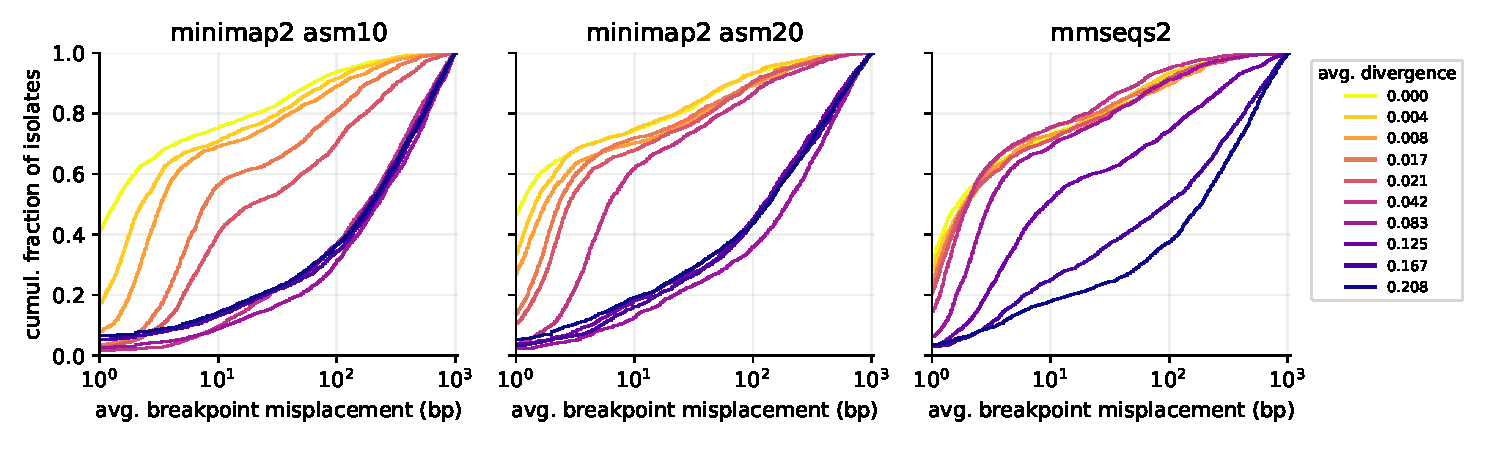
\includegraphics[width=\textwidth]{figs_suppl/accuracy_comparison.pdf}
    \caption{{\bf Accuracy of PanGraph algorithm on synthetic data}.}
    \label{fig:benchmark-accuracy-suppl}
\end{figure}

\section{Benchmark of \textit{PanGraph} on real data}

\begin{figure}[h]
    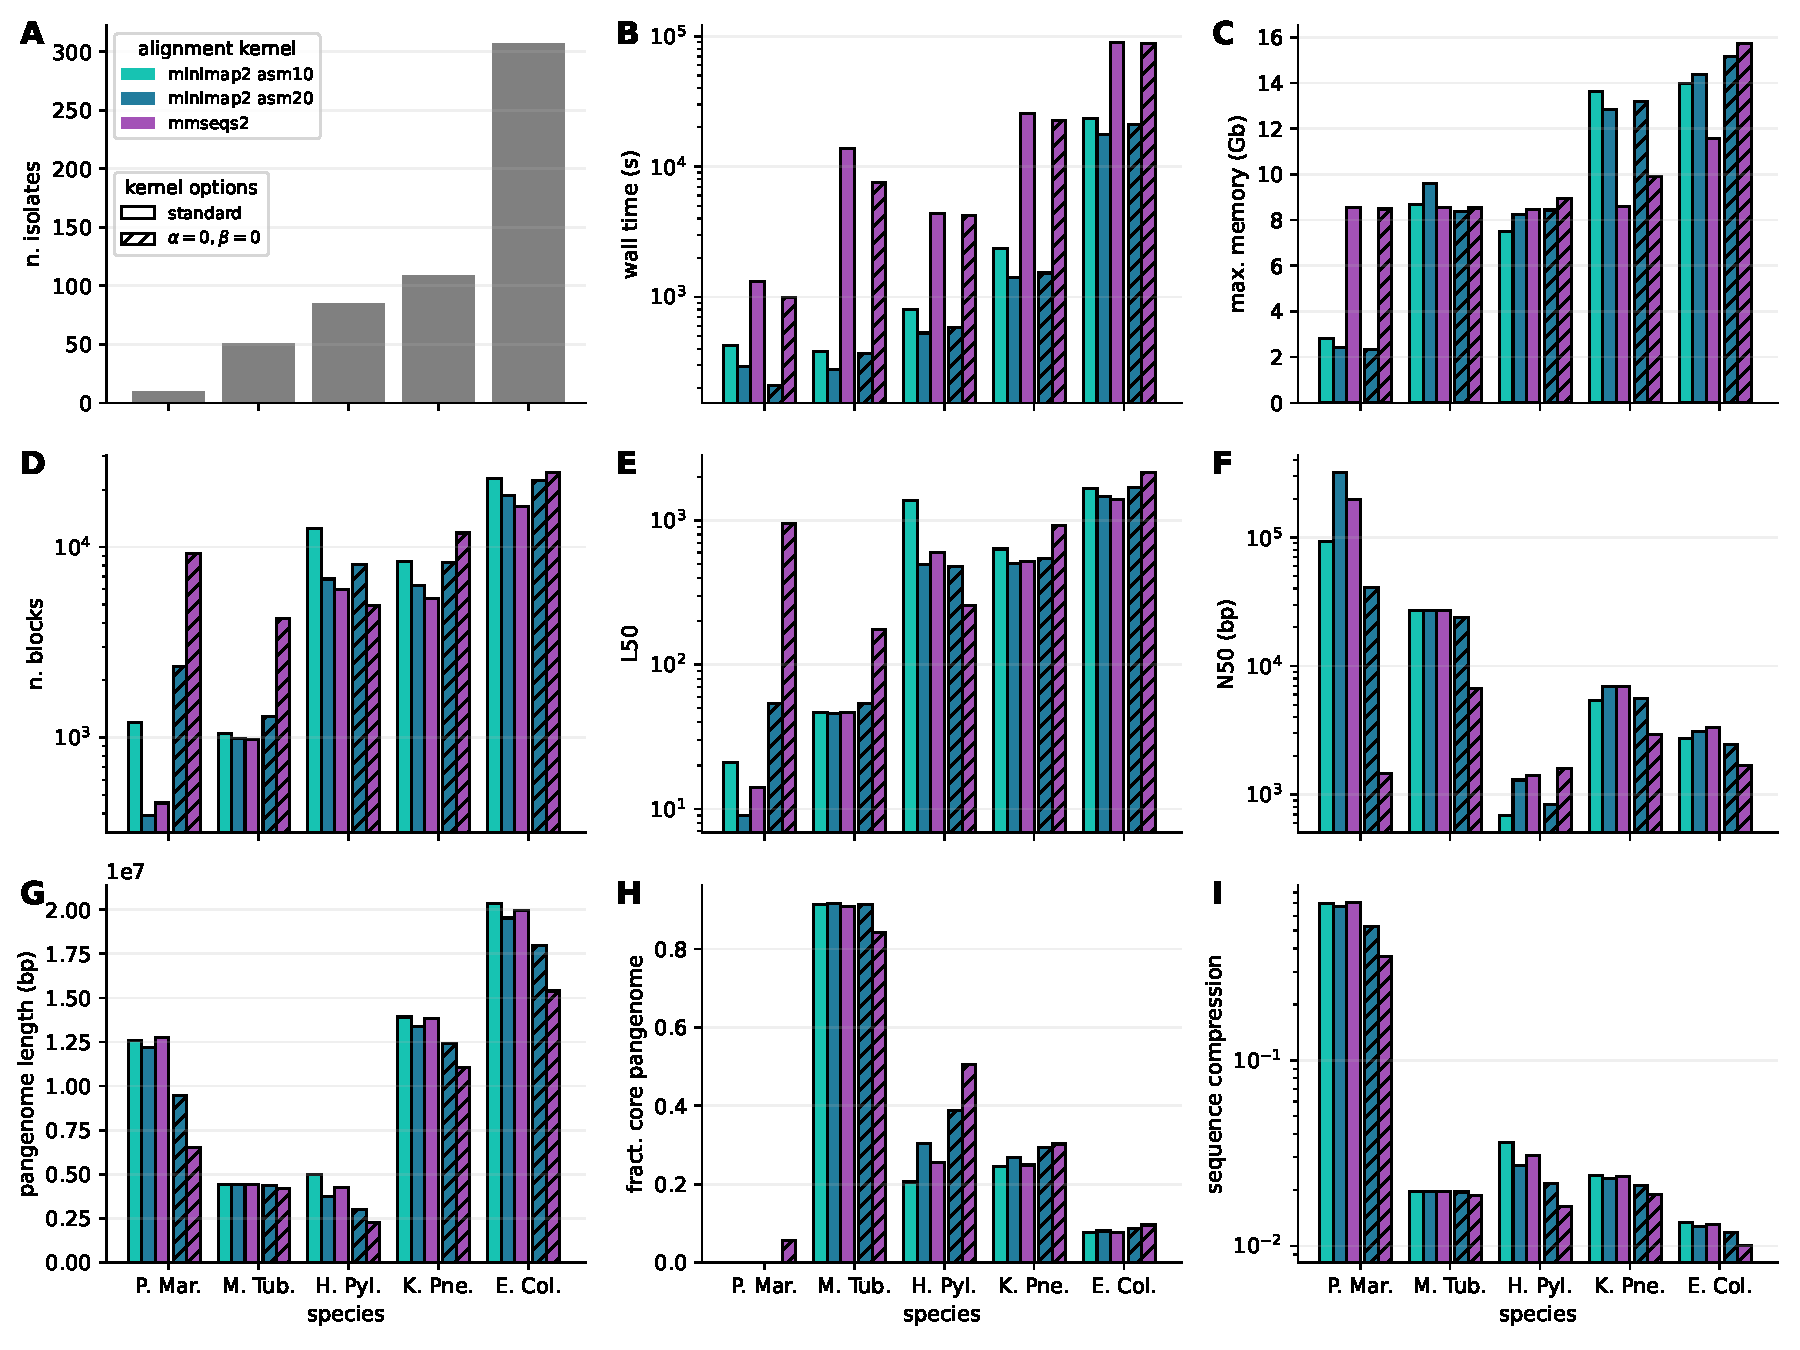
\includegraphics[width=\textwidth]{figs_suppl/panx_benchmark_suppl.pdf}
    \caption{{\bf Benchmark on real data}.}
    \label{fig:panx-benchmark-suppl}
\end{figure}


\section{Graph marginalization}

Given a graph composed of many different genomes, PanGraph is capable of marginalizing this graph on a subset of strains with the \verb|marginalize| command. To test this feature we built pangenome graphs on genomes from 5 different species: \textit{Klebsiella Pneumoniae} (KP), \textit{Helicobacter Pylori} (HP), \textit{Prochlorococcus Marinus} (PM), \textit{Mycobacterium Tuberculosis} (MT) and \textit{Escherichia Coli} (EC), extracted from RefSeq.\footnote{The list of accession numbers for each species and pairs is available on the repository: \url{https://github.com/neherlab/pangraph/blob/feat/finalize-paper/script/config/projection_strains.json}} For each strain we took 50 different strains (10 for PM) and built an unique pangenome graph using the \verb|build| command with standard values of the parameters. For each species we then randomly picked 50 different pairs of strains (45 for PM) and extracted the corresponding sub-graphs using the \verb|marginalize| command. We compared each of these graphs to their counterpart generated simply by using the \verb|build| command on the corresponding pair of strains.\\
The comparison between the marginalized (MG) and pairwise (PW) graph consists in splitting each genome using the overlap of the breakpoints given by the two different graphs. Then for each resulting segment we check whether it is shared with the other strain of the pair on either of the graphs. This gives raise to four different possibilities, corresponding to the segment being shared (1) or not (0) on either of the two graphs (MG/PW). We consider four different classes of segments: \textit{agree on sharing} (1-1 or 0-0), \textit{shared on both} (1-1), \textit{private on both} (0-0) and \textit{disagree on sharing} (1-0 or 0-1). For each class we measure the total and average length of the segments belonging to that class, and display the results in Fig.~\ref{fig:marginalize-suppl}.\\
For all species except for PM we find that MG graphs are compatible with their PW counterpart: segments on which the graphs \textit{disagree on sharing} represent only a minor fraction of the genome (much smaller than the fraction of shared or private segments) and their size is compatible with the default block length threshold of PanGraph (100 bp). PM represents and exception, with the great majority of segments being private on each graph and having large size. This expected since for PM the strains considered are highly diverged, above the sensitivity of minimap2 ($\sim 27\%$ core divergence). This causes the majority of blocks not to be merged, and generates a strong order dependence. The size of segments with \textit{disagreement on sharing} is also the largest, some segments having size of 10s of kbp.

\begin{figure}[h]
    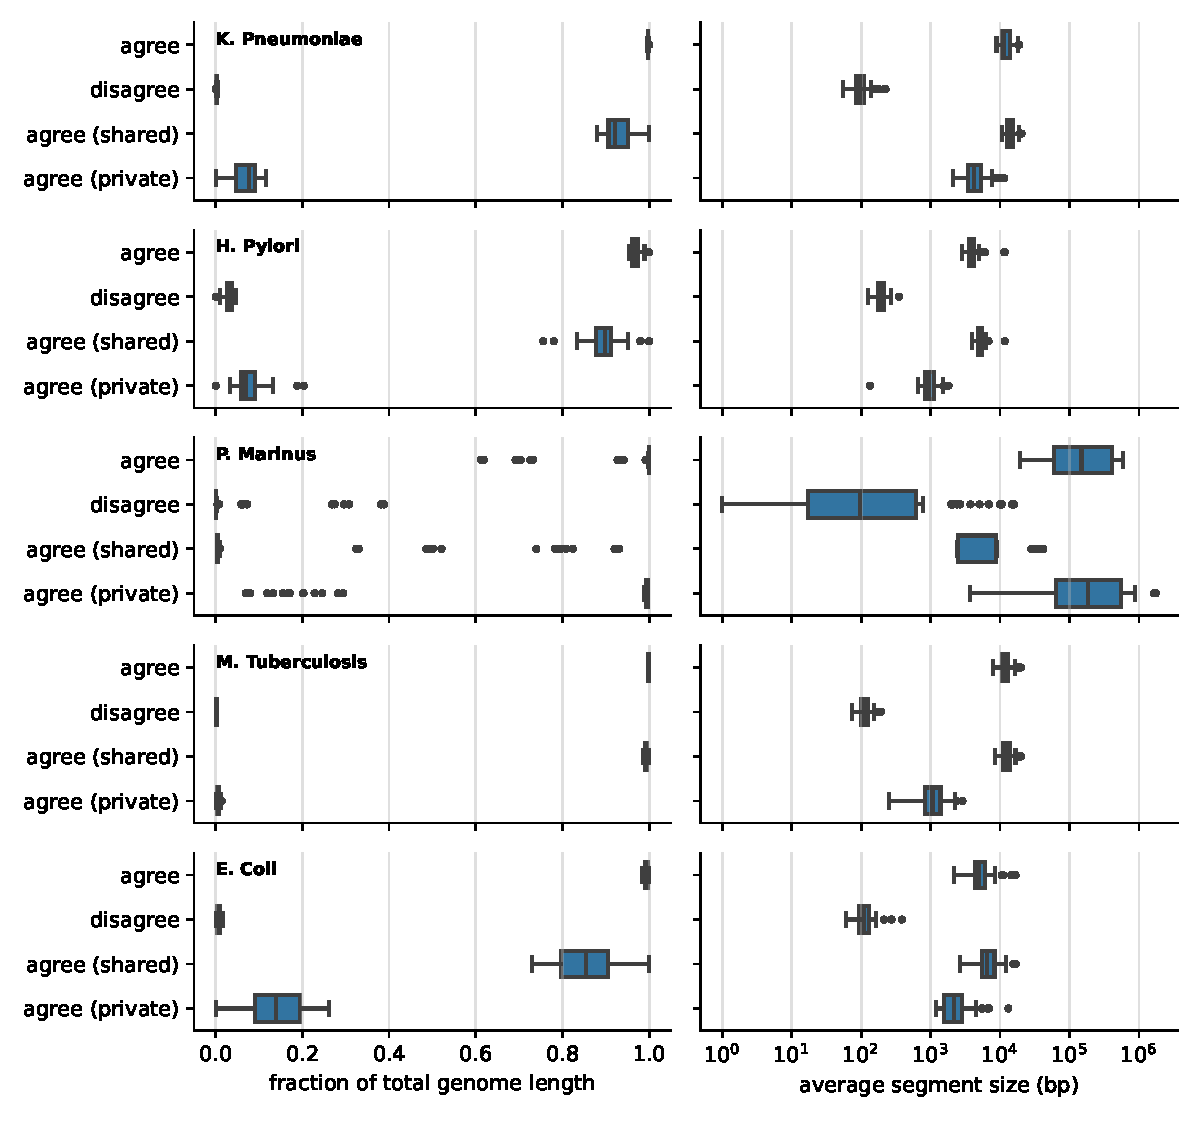
\includegraphics[width=.8\textwidth]{figs_suppl/proj_fig.pdf}
    \caption{{\bf Marginalized graphs are compatible with pairwise graphs}. Comparison of marginalized (MG) and pairwise (PW) built graphs for 5 different species. For each pair of strains we measure the length of segments in which MG and PW graphs agree on whether the segments are shared on both strains (\textit{agree on sharing}). These can either be both shared (\textit{shared on both}) or both private (\textit{private on both}). We also measure the length of segments on which the MG and PW graphs disagree (\textit{disagree on sharing}). For each of these for cases we report the total length as fraction of the average genome (left column) and the average size of each segment (right column). For each category we display the distribution of average results for 50 different pairs (45 for PM).
    }
    \label{fig:marginalize-suppl}
\end{figure}

\bibliography{cite}{}

\end{document}